\chapter{HISTORY AND ACKNOWLEDGEMENTS}
% !TEX root = hazy2.tex

\section{History}

\Cloudy\ was born at the Institute of Astronomy, Cambridge, in August of
1978, in the computing environment described in the web document
\href{http://www.nublado.org/gary/computing1970s.htm}{http://www.nublado.org/gary/computing1970s.htm}.  Its development has been
continued at The University of Kentucky, The Ohio State University, and
during extended visits to the Joint Institute for Laboratory Astrophysics,
the Royal Greenwich Observatory, IOA Cambridge, Cerro Tololo Interamerican
Observatory, and the Canadian Institute for Theoretical Astrophysics.

The code has been through three computer languages.  It was originally
written in FORTRAN IV and advanced through several dialects,
reaching FORTRAN
77  in 1994 (version 84). Version 90 was written in a mix of FORTRAN 77
and MILSPEC extensions.  This was the most advanced Fortran that could be
used with open source compilers.  It moved to ANSI 89 C in 1999 (version
96) and to C++ with the release of 07.02 in 2007.

Moore's Law is due to Gordon Moore, one of the founders of Intel
Corporation.  He observed that modern CPU's become about twice as powerful
every 18 months.  This trend has held true for the past twenty years, shows
no sign of failing, and seems to be associated with our ability to control
complexity.  By this standard the growth of \Cloudy\ has been conservative,
in that it is growing slower and complex on the Moore's-law timescale.
Figure \ref{fig:size} shows the evolution of the code,
as indicated by its size as a
function of time.\footnote{Before mid-1995 the size was the total number of lines in the
distributed source.  After 1995 the size only includes the number of lines
excluding block data.  When the code was converted to C the block data
were converted to external data files.  These external files are now far
larger than the code itself.}
As another example, the Meudon 1985 Meeting planetary
nebula test (\cdCommand{pn\_paris.in} in the test cases)
has always taken about one minute to compute.

\begin{figure}
\centering
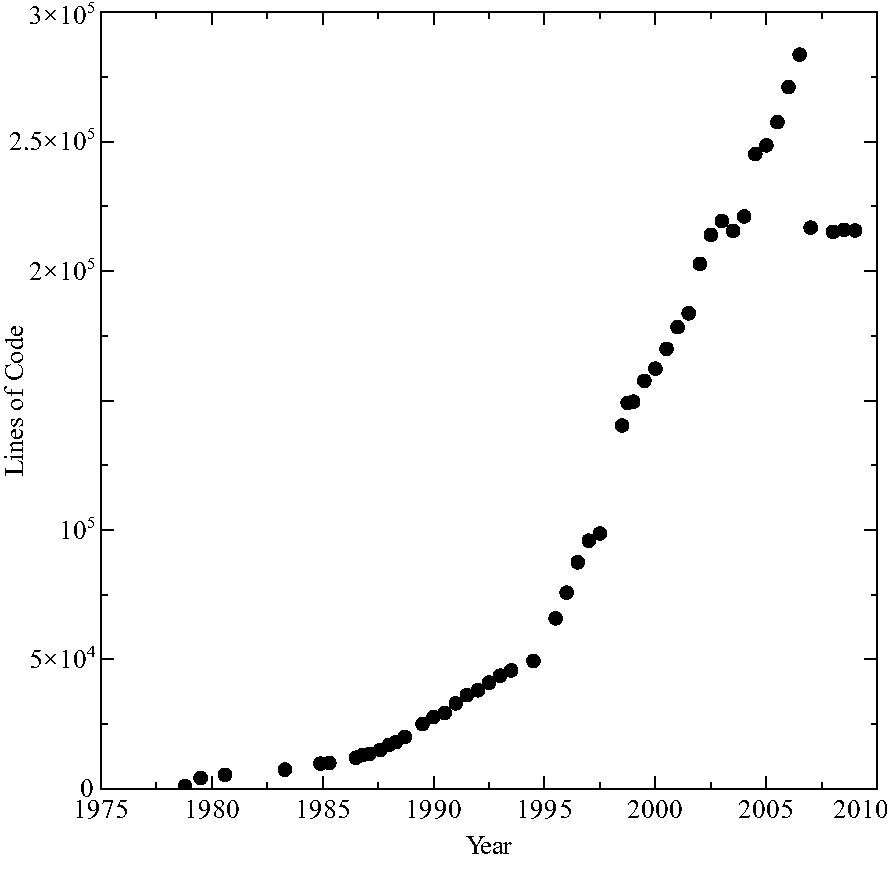
\includegraphics{size}
\caption[\protect\Cloudy's size vs time]{\label{fig:size}The size of the code as a function of time. The code grows roughly
7\% larger per year, with growth spurts and slowdowns at times. There are
several changes in slope evident - the year and cause are: 1985 - mainframe
to Unix; 1993 - Unix to windows; the jump at 1999 - the Fortran to C
conversion and the Williams / van Hoof drop in 2006, due to the use of
object-like structures and moving converted fortran block data into separate
files.}
\end{figure}

\section{Acknowledgments}

Comments or suggestions which led to the improvement of \Cloudy\ were made
by the many individuals acknowledged on the web site
\href{http://www.nublado.org}{http://www.nublado.org}.

Peter G. Martin and Hagai Netzer had special roles during the early
development of the code.  Peter added several of the commands that deal
with ordering of supplemental line lists and the luminosity options on the
\cdCommand{blackbody} command, insisted that \Cloudy\ run on a VAX, provided access to
the University of Toronto VAX 11/780 during the 1980's, and more recently
hosted the group at CITA during a sabbatical.  Hagai and I have spent
countless hours arguing over methods, assumptions, and just whose code had
the bug.  These comparisons are the only way to debug codes as large as
\Cloudy\ or ION.

Peter van Hoof has gone over the code very carefully, finding many
problems, and expanding its capabilities.  The current version of the grain
physics was developed by Peter together with Peter Martin, and Joe
Weingartner.  PvH developed the stellar library implementation in the current
version.  He is the maintainer for both the grains and stellar atmospheres
codes.

The move to make the solvers far more rigorous and include dynamics and
advection has been led by Robin Williams and Will Henney.  Robin has
rewritten the chemistry solvers to take advantage of the structures present
in the C language and make them more robust.

The initial implementation of the hydrogen iso-electronic sequence was
done by Jason Ferguson as part of his thesis. Ryan Porter developed the
He-like isoelectronic sequence in his thesis. The expansion of the
simulations into the PDR was done by Nick Abel and Gargi Shaw as part of
their theses.

Sections of the code are taken from public domain software, as
acknowledged in this document and in the source.
Portions of the code were written by those listed in the
\cdFilename{others.txt} file in the distributed files.

The preparation of the bibliographic references in this document made
use of data from the NASA's Astrophysics Data System Bibliographic
Services.

The development of \Cloudy\ would not have been possible without
twenty nine years of continuous support by The National Science
Foundation.  This began with AST 80-2522, and has been continued with
grants 83-05094, 85-12414, 87-19607, 90-19692, 93-19034, 96-17083,
00-71180, 03-0772, and most recently AST 06-07028.  NASA has supported
\Cloudy\ through ATP program awards NAG5-12020 and NNG05GD81G.
Support from the University of Kentucky Center for Computational
Sciences is also gratefully acknowledged.

